Dans les chapitres précédants, les bases théoriques sur les automates et languages ont été introduites. Celles-ci ont été suivies de concepts plus étroitement liés à LeVer tels que les automates à files, les traces, traces annotées et languages associés. Un dernier élément présenté dans la section \ref{sec:unsafe} est la sécurité d'un état ou d'un automate.

En appliquant l'algorithme d'Angluin \cite{Angluin87} selon la méthode LeVer \cite{Vardhan04}, il est possible de se prononcer sur la sécurité pour toute une classe d'automates à files : ceux pour lesquels le language de traces annotées est régulier.

L'objectif dès lors n'est pas d'apprendre le language de l'automate à file mais le language de trace associé, et d'adapter la méthode pour répondre à la question de sécurité. En formulant les bonnes propriétés, il est également possible d'interrompre l'algorithme d'apprentissage avant terme si l'on peut se prononcer sur la sécurité de façon certaine.


\begin{figure}[H]
	\centering
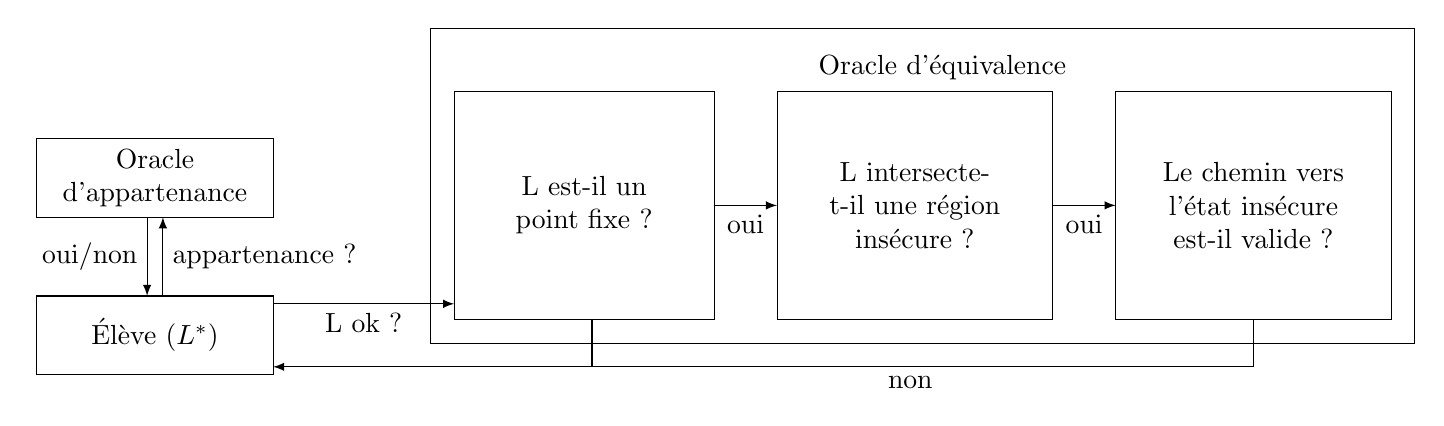
\begin{tikzpicture}
	\tikzset{>=latex}

  \draw (0,-3.4) rectangle (3,-4.4) node[pos=.5] {Élève ($L^*$)};
  \draw (5,0) rectangle (17.5,-4);
	\draw[->] (3,-3.5) -- (5.3,-3.5) node[pos=0.5,below] {L ok ?};

  \draw (0,-1.4) rectangle (3,-2.4) node[pos=.5,text width=3cm,align=center] {Oracle\\ d'appartenance};
  \draw[->] (1.6,-3.4) -- (1.6,-2.4) node[pos=0.5,right] {appartenance ?};
  \draw[<-] (1.4,-3.4) -- (1.4,-2.4) node[pos=0.5,left] {oui/non};

  \node[draw=none] at (11.5, -0.5) {Oracle d'équivalence};

  \draw (5.3, -0.8) rectangle (8.6, -3.7) node[pos=0.5,text width=3cm,align=center] {L est-il un point fixe ?};
  \draw (9.4, -0.8) rectangle (12.9, -3.7) node[pos=0.5,text width=3cm,align=center] {L intersecte-t-il une région insécure ?};
  \draw (13.7, -0.8) rectangle (17.2, -3.7) node[pos=0.5,text width=3cm,align=center] {Le chemin vers l'état insécure est-il valide ?};

  \draw[->] (8.6, -2.25) -- (9.4,-2.25) node[pos=0.5,below] {oui};
  \draw[->] (12.9, -2.25) -- (13.7,-2.25) node[pos=0.5,below] {oui};
  \draw[->] (15.45, -4.3) -- (3, -4.3) node[pos=0.35,below] {non};
  \draw[-] (7.05, -3.7) -- (7.05, -4.3);
  \draw[-] (15.45, -3.7) -- (15.45, -4.3);


\end{tikzpicture}
\caption{Vue schématique de l'algorithme d'Angluin}
\end{figure}


\todo{Ce chapitre décrit le fonctionnement de LeVer en se basant sur tout le reste. Concrètement, il s'agit d'une reformulation de l'algorithme d'Angluin pour les automates FIFO selon la méthode de Vardhan}

\todo{Cette section explique le but recherché, son importance et la structure du chapitre}
